\documentclass[a5paper,
              twoside,
              headings=small,
              titlepage=firstiscover,
              numbers=noenddot]{scrbook}

\usepackage[sjannon] {ofs}\OFSfamilydefault [JannonTModerne]

\usepackage[english]{babel}
\usepackage[utf8]{inputenc}
\usepackage[T1]{fontenc}

\usepackage{graphicx}
\usepackage{url}

\usepackage{csquotes}

\usepackage{tikz}
\usetikzlibrary{shadows}

\setcounter{figure}{0}
\renewcommand{\thefigure}{\arabic{figure}}

\newcommand*\keystroke[1]{%
  \tikz[baseline=(key.base)]
    \node[%
      draw,
      fill=white,
      drop shadow={shadow xshift=0.25ex,shadow yshift=-0.25ex,fill=black,opacity=0.75},
      rectangle,
      rounded corners=2pt,
      inner sep=1pt,
      line width=0.5pt,
      font=\scriptsize\sffamily
    ](key) {#1\strut}
  ;
}

%
% Počet stran dělitelný 4 kvůli sazbě!
%

\begin{document}

\title{Fedora Workstation}
\subtitle{An Introduction and First Steps Guide}
\date{}
\maketitle

\cleardoublepage

\chapter*{Introduction}
So, you've decided to install the \emph{Fedora Workstation} operating system on your workstation, desktop, laptop, netbook\dots or any other kind of a PC. How should you proceed? What are the benefits of \emph{Fedora Workstation} as compared to other operating systems? How do you get it and install it? How do you tweak it to your taste and for your particular needs? In this guide we will examine each of these questions, step by step.


\chapter*{What Is Fedora About}
\section*{Who Is It For?}

Fedora is available in several different editions, each targeted at different kinds of users. The \emph{Fedora~Workstation} edition this handbook is about is designed for users who use computers primarily to create, from developers to graphic designers, musicians, and writers.

\emph{Fedora~Workstation} features the~\emph{GNOME~3} environment and a variety of tools for developers (like the newly released \emph{Builder}), \sloppy{applications for virtualization (\emph{Boxes}), container management tools (\emph{Docker}), and many more.} But it is definitely not just for developers and engineers! It also comes with several tools for video editing (\emph{PiTiVi}), audio editing (\emph{Audacity}), as well as for editing bitmap (\emph{GIMP}), vector (\emph{Inkscape}), and 3D (\emph{Blender}) graphics.

In a sense, \emph{Fedora~Workstation} is a better operating system for an average user than it ever was.

\section*{Open Source and Freedom}

Open source software is software that has made its source code available for distribution, modification, and use for any purpose. Fedora has been created and maintained for over 10~years by a community of professional developers and volunteers who are passionate about open source and because of it, it has always included and will continue to include only open source software. It doesn't include any software that can't be reviewed at the source code level.

At the same time, Fedora doesn't prevent you from installing any software you want. Do you want a non-open source application, such as \emph{Google Chrome}? You can easily install it. But, even without 3rd-party and non-open source software, you'll find more then 20,000 packages for Fedora which represent various applications, extensions, and libraries. Many of these open source programs are not just alternatives, but are often better or more powerful than their closed source counterparts. For more information, see the \emph{Installing New Software} chapter.

Fedora is, however, not just about open source, but is also passionate about freedom in the form of software licenses and patents. Fedora respects software patent law (even though it may not be relevant in some parts of the world). You can be sure that you are not breaking laws by using Fedora.

\section*{Security and Privacy}

Fedora development prioritizes security and includes clear rules to ensure that it remains its primary focus. Like any other significant software product, each release is carefully tested. Moreover, Fedora is the base for Red~Hat~Enterprise~Linux, a commercially supported operating system offered by Red~Hat. Red~Hat employs a lot of developers, many of whom are involved in the Fedora Project, and owns Fedora trademarks.

The Fedora community support lasts for two release cycles plus one month. This means that with a new release every 6 months, each version of Fedora is supported for 13~months. The Fedora community support includes security fixes and kernel updates, which is significant because new kernels mean improved and new hardware support. This is a big advantage of using Fedora.

The Fedora community carefully selects the software to include in the operating system and is concerned about privacy. Therefore, Fedora doesn't include any programs that send any sensitive data without your permission. Fedora doesn't spy on you, it respects your privacy.

\section*{Leading the Way}

Fedora integrates a lot of new software and is often the first (or one of the first) operating systems to adopt new technology. Fedora is very often where new technologies are being developed and tested.

Open source software is about collaboration and people who are involved in the Fedora Project are very often active in other projects, too. They don't wait until someone else develops software so they can include it in Fedora. Instead they actively participate in the project's development and collaborate with participants from other Linux operating systems or independent developers. It is common that such software goes on to become the de facto standard of the Linux world.

Fedora users keep fingers on the pulse of innovation and change and are ahead of others. This is why it is easy to say that Fedora is progressive, innovative, and leading the way.

\section*{How to Get Fedora?}
\subsection*{Getting Fedora}

You can install Fedora from optical media (CD, DVD), a USB flash drive, or over the network by using an appropriate installation image. Installation images of \emph{Fedora~Workstation} are available for download in the ISO format at \url{http://getfedora.org}. \emph{Fedora Workstation} defaults to a 64-bit operating system download as that is what is best for most users.

If you aren't ready to install Fedora yet and would like to try it first without losing or changing anything already on your PC, make sure you download a live image. With this image, you can boot to a fully functional system and find out what Fedora is like, experiment with it, and determine whether it fully supports your PC's hardware.

To run \emph{Fedora Workstation} reasonably well it is recommend that you have at least a 1~GHz processor, 2~GiB of memory, 10~GiB of hard drive space, and a graphics card that supports hardware acceleration. These aren't the minimum requirements, but they are the best for most users. Some users may wish to run Fedora on lower powered machines and will find it performs well there too.

\subsection*{Creating Installation Media}

In order to install or run Fedora from an installation image, you need to create installation media first:
\begin{itemize}
\item\emph{USB Installation} -- To create a USB installation drive, you can use the \emph{Fedora Media Writer}. It can run on \emph{MS Windows}, \emph{Apple macOS} or Linux. Beware, this program will erase all the data on the flash drive! \emph{Fedora Media Writer} can download the installation image for you when you run it. If you're using \emph{MS Windows} or \emph{Apple macOS}, the installation file of the application is what you'll be offered when you decide to download \emph{Fedora Workstation} at \url{https://getfedora.org}.

\emph{GNOME and Disks} -- If you already use a Linux operating system with the GNOME desktop environment, you can use built-in software to write to a USB drive. In the \emph{Files} application, right-click an ISO image, choose "Open in a different app" and then choose "Write on disk". This will open the \emph{Disks} utility which will write the image on to a flash drive.

If you decide to write the installation image on to a USB flash drive, carefully double-check that you've picked the correct target drive. If you're doing this on \emph{MS Windows}, you need to pick the character that has been assigned to the drive you'd like to use (typically this will be \texttt{D:} or \texttt{E:}). On Linux, you need to do the same using the device (typically this is will be \texttt{/dev/sdX} where \texttt{X} is an alphabetic character). The easiest and safest way to do this on Linux is to use the \emph{Disks} utility mentioned above.

\item\emph{DVD Installation} -- Using a \emph{DVD} is a very traditional way of installing Fedora. You can create an installation DVD by writing an ISO image to a DVD. Most modern operating systems can do this operation with built-in software. If not, you can install a specialized application such as \emph{Brasero} on Linux and \emph{ImgBurn} on \emph{MS Windows}. All versions of \emph{Apple macOS} can write DVDs using \emph{Finder} and \emph{Disk Utility}.
\end{itemize}

\subsection*{Installing Fedora}
\begin{enumerate}
\item\emph{Booting} -- No matter what media you've chosen, you'll need to make sure that you set the right boot sequence in the BIOS of the computer you'd like to install Fedora~Workstation\footnote{just Fedora?} on. The drive with the install media needs to be in the first position. You can get to the BIOS configuration by pressing a specific key after starting the computer. The key depends on the vendor (typically the keys are \keystroke{Delete}, \keystroke{F1}, or \keystroke{F2}). Alternately, many vendors allow you to choose a boot drive without having to go to the BIOS settings by pressing the \keystroke{F12} key.

\item\emph{Initial Screen} -- After successfully booting from the installation media, you'll see the initial screen where you can choose between installing Fedora~Workstation\footnote{just Fedora?} (or booting into the live system) and verifying the install media. If you choose installation, you'll boot into the live system and will be asked if you want to try the system out or install it on the hard drive. If you choose to "Try Fedora" you can use it in this way for as long as you want and can choose to perform an installation at any time by clicking on the installer icon in the menu.

\begin{figure}[ht]
\begin{center}
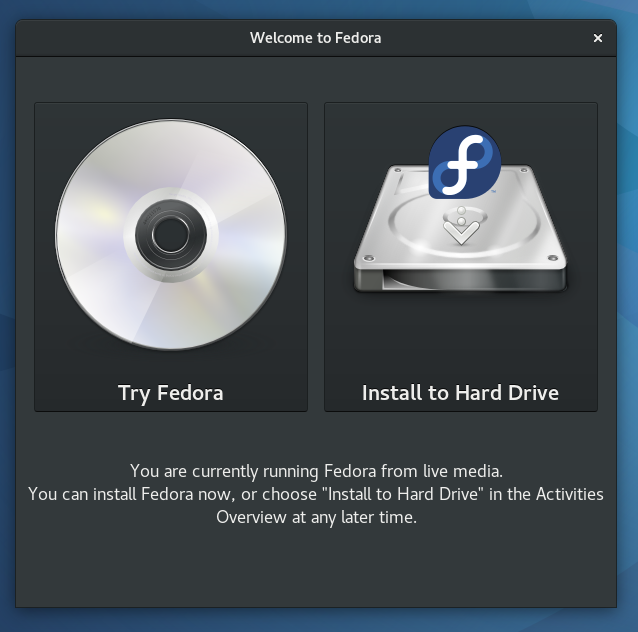
\includegraphics[width=.75\textwidth]{img/installer-a}
\captionbelow{Booted installation media of Fedora Workstation} \label{fig:installer-a}
\end{center}
\end{figure}

\item\emph{Trying the System} -- If you've chosen to try the system, you'll begin using the \emph{GNOME~Shell}. The top of the display contains the most commonly used control elements. There is an \emph{Activities} button in the upper left corner which will get you to applications (and to the option to install \emph{Fedora~Workstation}\footnote{just Fedora?} on your system). The upper right corner has controls that allow you to set up the network, as well as to restart or shut down the system.

\item\emph{Installer} -- Once you decide to install Fedora Workstation\footnote{just Fedora?}, you'll being using the installation program, Anaconda. The installer consists of different spokes that manage the options for areas such as language settings, time zone, etc.

\begin{figure}[ht]
\begin{center}
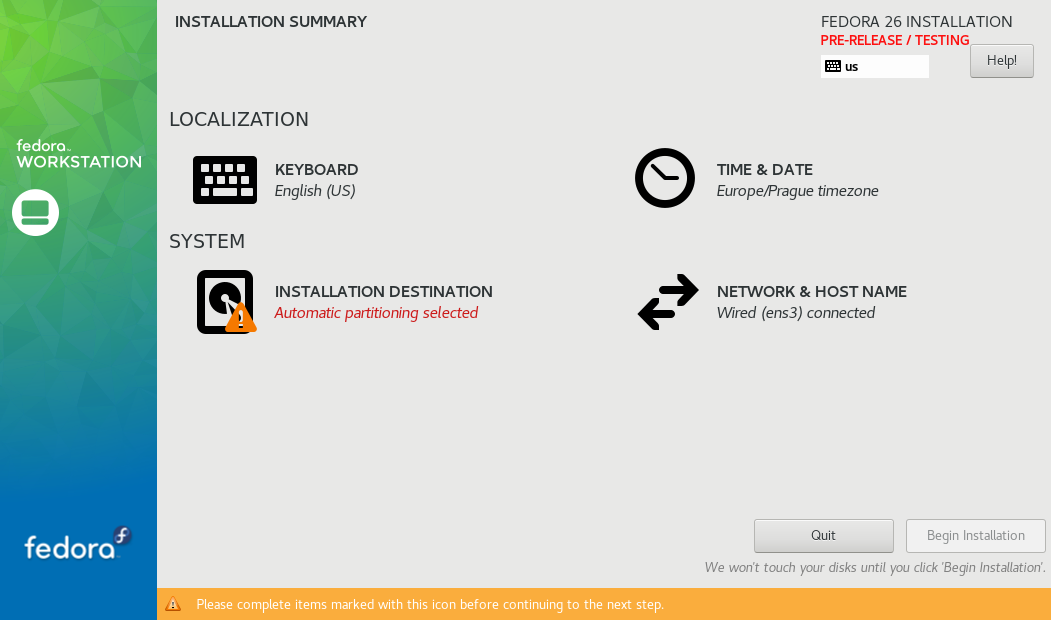
\includegraphics[width=0.95\textwidth]{img/installer-b}
\captionbelow{Fedora Workstation Installer} \label{fig:installer-b}
\end{center}
\end{figure}

The disk partitioning spoke is the most important part of the installer. This spoke will define where on your hard drive Fedora Workstation\footnote{just Fedora?} will be installed. The installer offers you automatic partitioning which will configure the hard drive in a way that is useful for most people, or you can also choose manual partitioning and apply a customized setting. It is also possible to set up encryption for better security.

Fedora Workstation\footnote{just Fedora?} also allows you to create a dualboot system, that is, to have two operating systems installed on your PC at the same time. It's easy to install Fedora Workstation next to an existing \emph{MS Windows} installation.

In the partitioning dialog, you will see the existing partitions on the left. Before you confirm the changes make sure that everything is the way you meant it to be (for example that all partitions of other operating systems are still there, if you wish to keep them). When you confirm the changes and start the installation, the changes will be final.

\item\emph{Finishing the Installation} -- While the system is being installed, you need to provide several important pieces of information such as the root or administrator password and the information for creating a user account.

You will normally use the user account you created and only use the root password when you need to make a system-wide change. Fedora Workstation\footnote{just Fedora?} has the classic approach to user accounts where the root account is not disabled. However, if you do not want to remember passwords for two accounts, you can check the \emph{Admin} option when creating your user account. This enables the account to act as an administrator in vast majority of operations and avoids your having to use the root password often.
\end{enumerate}

And that's it. The whole installation should take less than several dozen minutes. After a restart you'll just need to perform a couple of short post-install tasks such as changing the boot order to the original state and then you're ready to go.

Everything worked well? Now you can start exploring Fedora Workstation\footnote{Just Fedora? Or cursive?}!

\endinput

\chapter*{First Steps in New System}
\section*{Getting Oriented}

You're now looking at the \emph{GNOME Shell} environment. The first thing you'll probably notice when you start working with \emph{GNOME Shell} for the first time is that application windows only have the \emph{Close} button. The GNOME desktop environment tries to be as simple as possible and because you can maximize windows by dragging them to the top of the screen, minimize them by dragging them away from the top of~the screen, or do both by double clicking the title bar, there is no need to have dedicated \emph{Minimize} and \emph{Maximize} buttons.

\bigskip

\begin{figure}[htbp]
\begin{center}
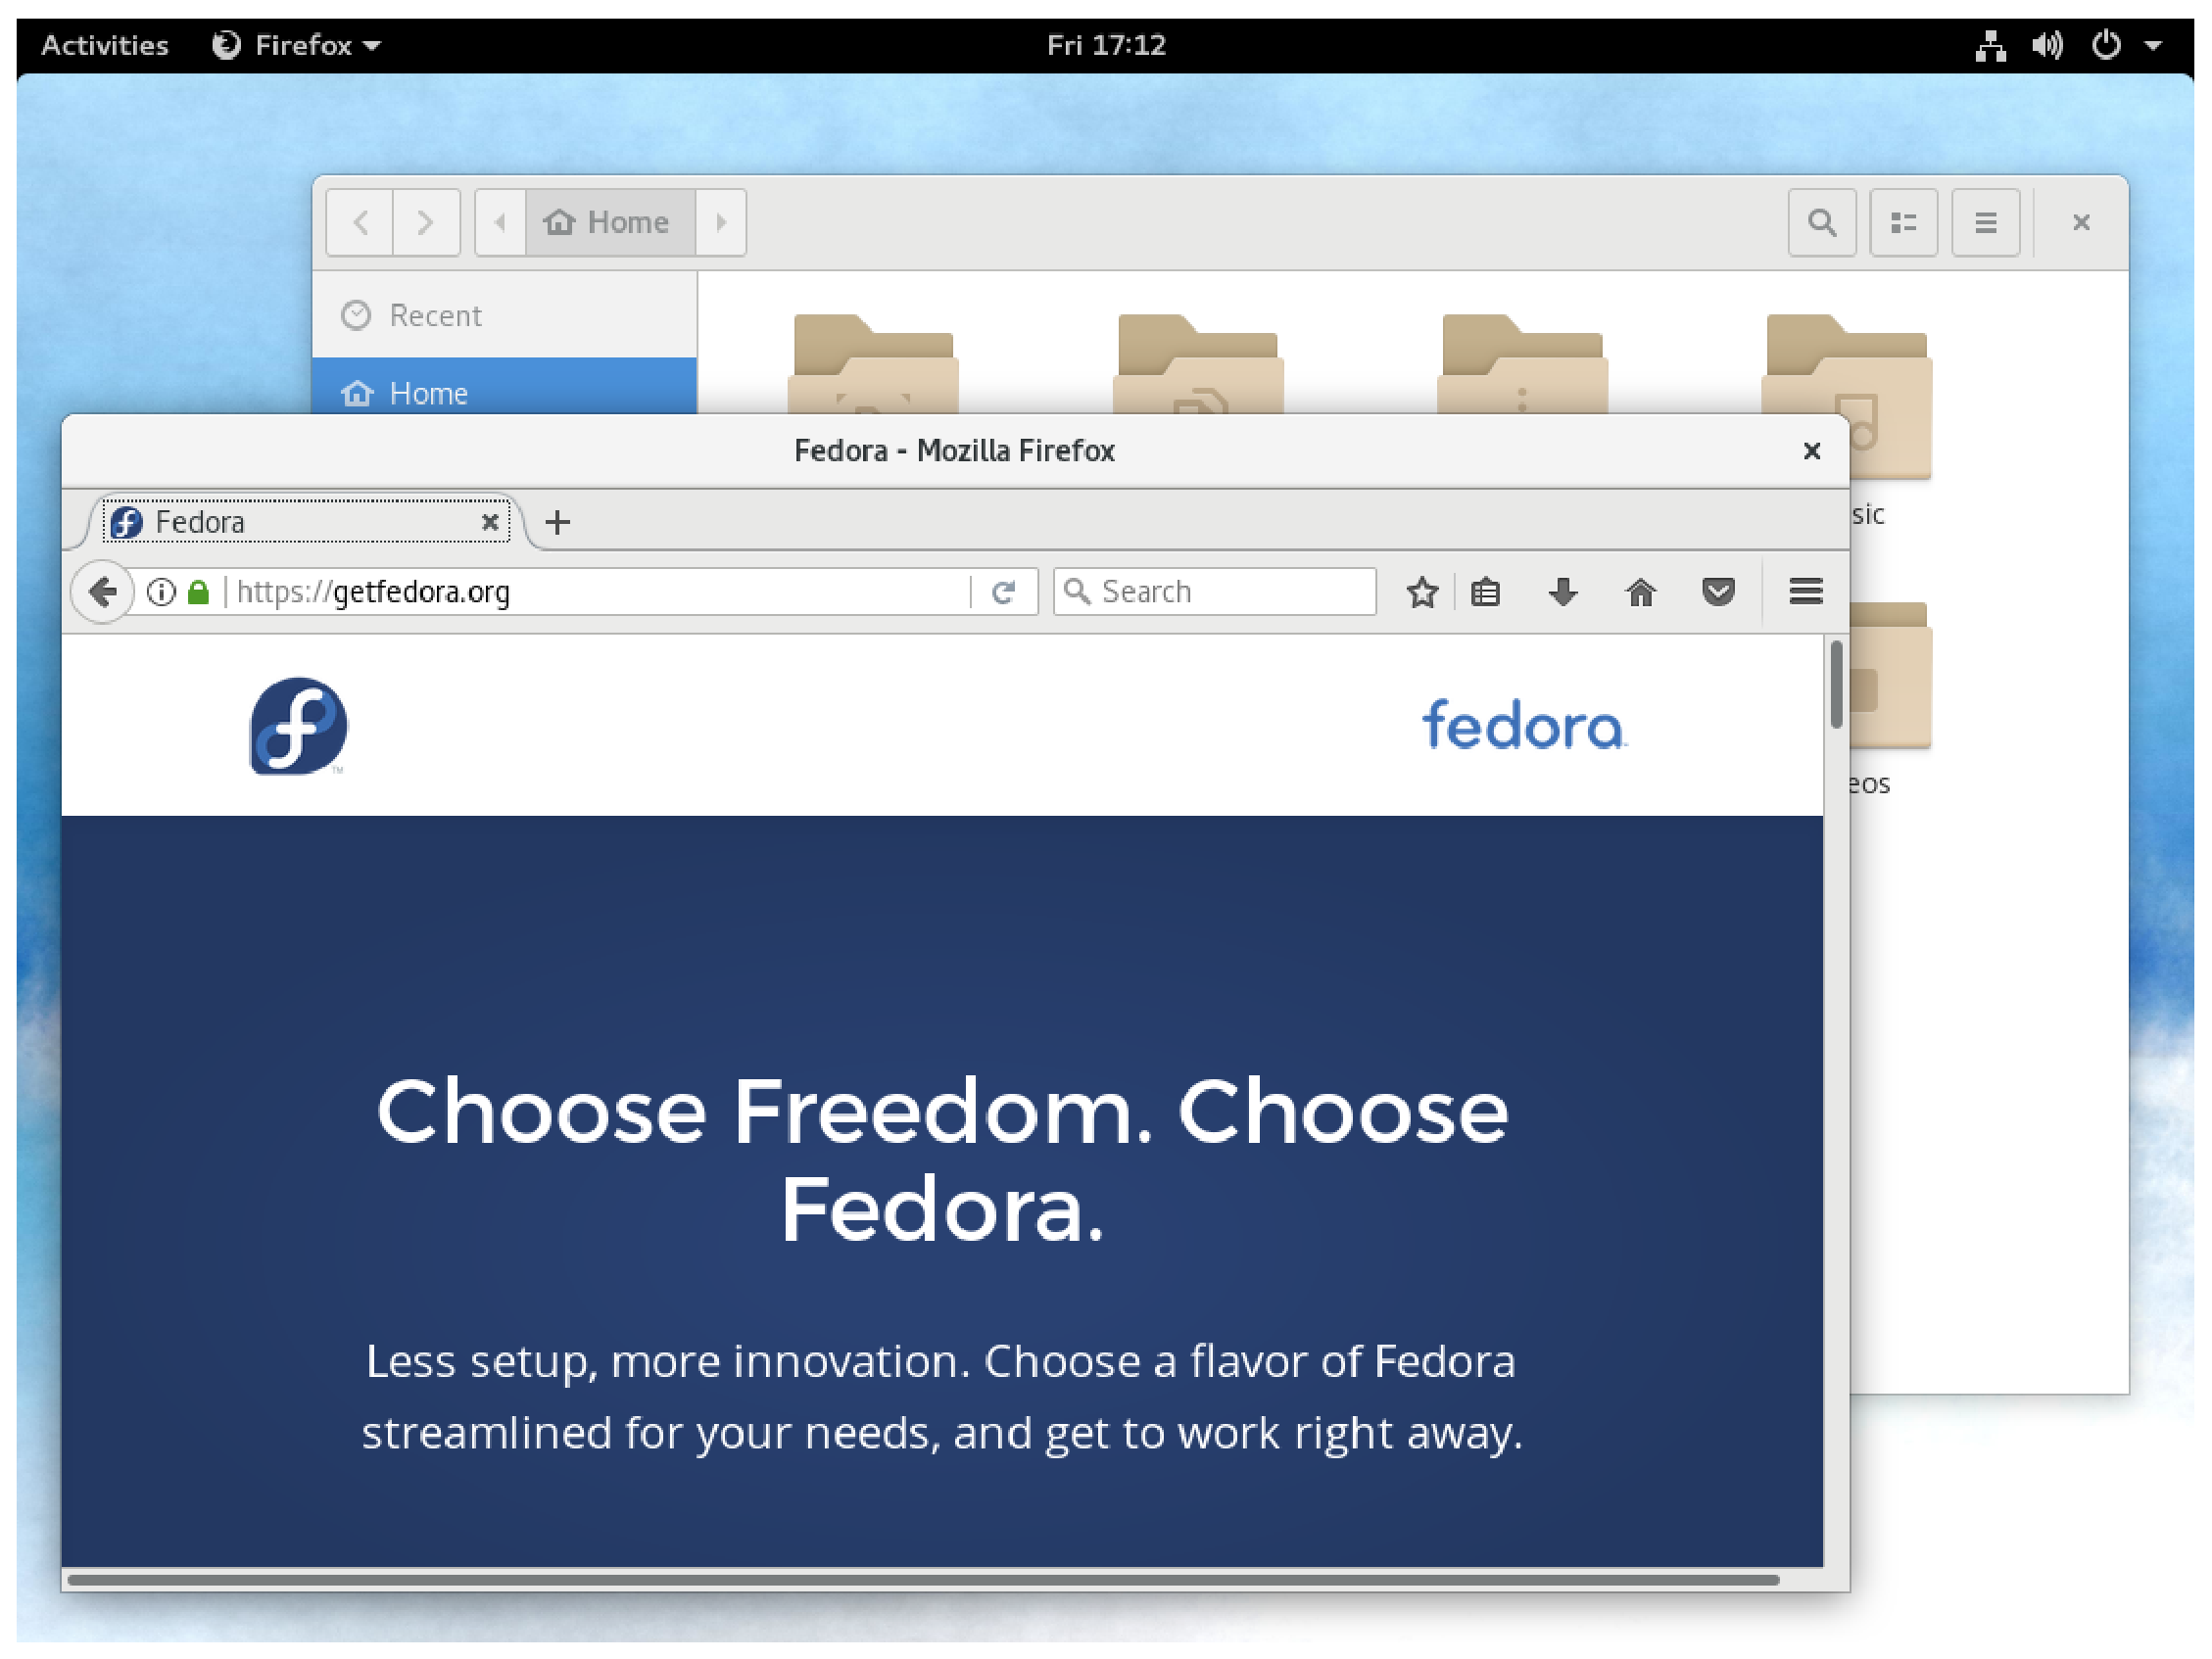
\includegraphics[width=0.75\textwidth]{img/shell-a}
\captionbelow{The initial screen of GNOME Shell} \label{fig:shell-a}
\end{center}
\end{figure}

\newpage
The top part of the screen includes the following items:
\begin{enumerate}
\item The \emph{Activities} button --- this button gives you access to the \emph{Activities Overview} and is the starting point for the majority of activities you typically expect from a desktop installation. We'll be taking a closer look at it in the next section.

\item The \emph{Clock and Calendar} applet --- clicking the current time in the top middle part of the screen gives you access to a list of missed notifications and also a calendar. If you use one of the applications that use the calendar back end of GNOME (such as \emph{Evolution}), you'll also see events you entered in those applications.

\begin{figure}[tbp]
\begin{center}
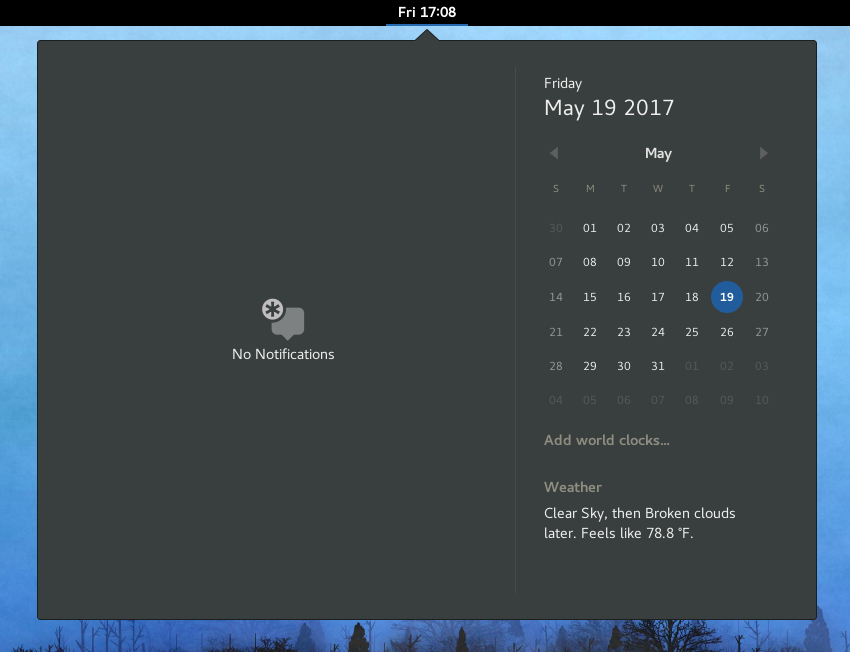
\includegraphics[width=0.75\textwidth]{img/calendar}
\captionbelow{The Clock and Calendar applet} \label{fig:calendar}
\end{center}
\end{figure}

\item The \emph{User Menu} --- in the upper right corner of the screen are located the most important indicators: the network connection status, the volume icon, and the battery status if you are using a laptop. Clicking on either of them will open a menu that will allow you to adjust the volume, change the brightness of your screen, select a suitable network connection option, connect to Bluetooth devices, and so on. Clicking on your name in this menu will give you an option to log out of the current session or switch to a different account. Finally, at the very bottom of this menu, you'll find three buttons: the left button will open the system settings, the middle button will lock the screen, and the right button will give you the option to restart or power off your machine.

\begin{figure}[tbp]
\begin{center}
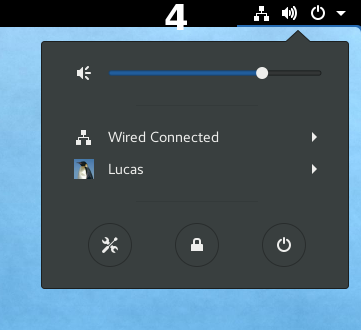
\includegraphics[width=0.45\textwidth]{img/menu}
\captionbelow{The User Menu} \label{fig:menu}
\end{center}
\end{figure}

\end{enumerate}

%\clearpage
\section*{Exploring the Activities Overview}

The key part of the user interface is the \emph{Activities} button located in the upper left corner of the screen. You don't even need to click it, just move the mouse pointer to the upper left corner or press the \keystroke{Super} key (also known as the \keystroke{Windows} key). When you do so, you will be presented with the \emph{Activities Overview} that will show you all currently open windows, give you access to installed applications, and allow you to switch between virtual workspaces.

\begin{figure}[t]
\begin{center}
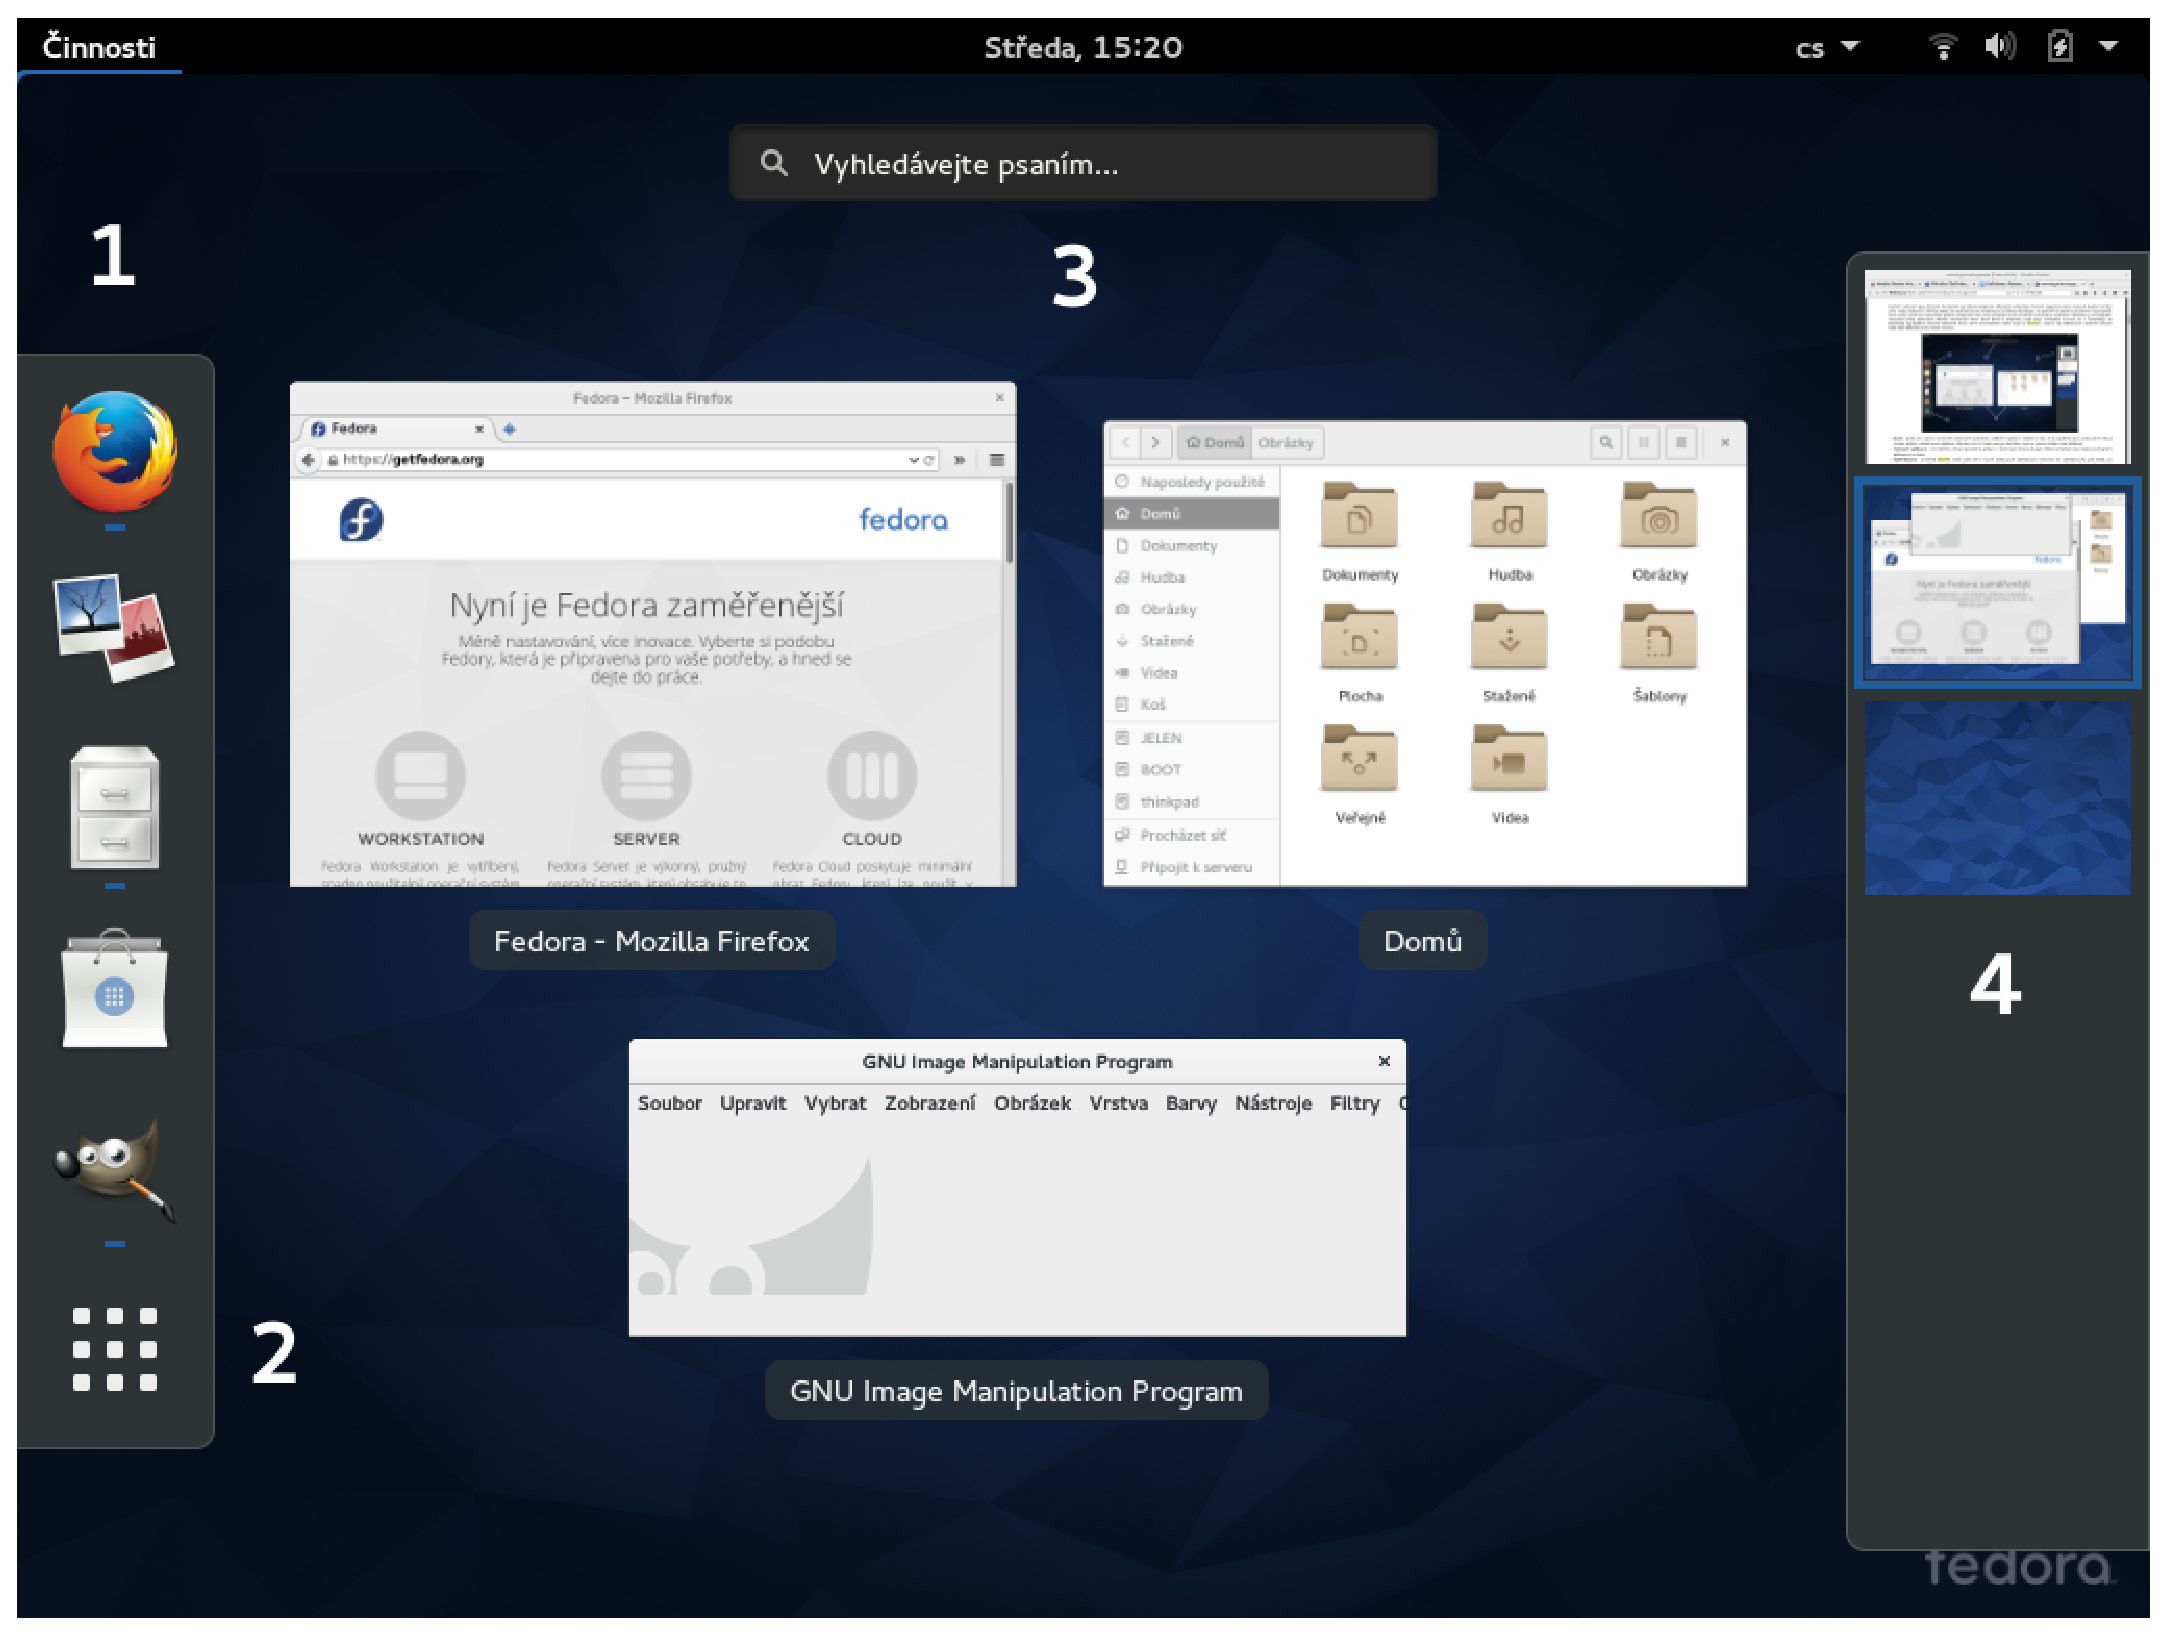
\includegraphics[width=0.93\textwidth]{img/shell-b}
\captionbelow{The Activities Overview} \label{fig:shell-b}
\end{center}
\end{figure}

The \emph{Activities Overview} consists of the following key components:
\begin{enumerate}
\item The \emph{Dash} --- the vertical panel along the left side of the screen gives you a quick access to all currently running applications and to those that you've marked as your favorite ones. Running applications are clearly underlined. If you want to mark a running application as your favorite, click its icon with the right mouse button and select \emph{Add to Favorites} from the menu.

\begin{figure}[t]
\begin{center}
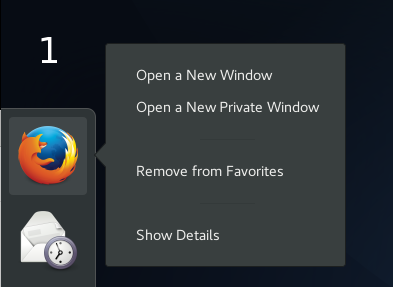
\includegraphics[width=0.42\textwidth]{img/dash-b}
\captionbelow{Working with applications in Dash} \label{fig:dash-b}
%\end{center}
%\end{figure}
\bigskip
%\begin{figure}[ht]
%\begin{center}

\includegraphics[width=0.42\textwidth]{img/dash-a}
\captionbelow{The Show Applications button} \label{fig:dash-a}
\end{center}
\end{figure}

\item The \emph{Show Applications} button --- \sloppy{at the bottom of the \emph{Dash}, you can find an icon depicting a grid of squares that says \enquote{Show Applications} when you move the mouse pointer over it. Click on it to get a list of application launchers. You can switch between launchers for frequently used applications and launchers for all installed applications by clicking the respective buttons at the bottom of the screen.}


\item The \emph{Search} field --- if you know the name of the application you're looking for or at least a part of it, after opening the \emph{Activities Overview}, you can just start typing the name and you don't even need to select the search field at the top of the screen. As you type, \emph{GNOME Shell} will not only show you all matching applications, but it will also offer you matching contacts, documents, pictures, settings, and so on. You can change what you want to include in the search results in the System Settings under \emph{Search}.

Using the \emph{Search} field is probably the fastest way to launch applications in GNOME.

\begin{figure}[ht]
\begin{center}
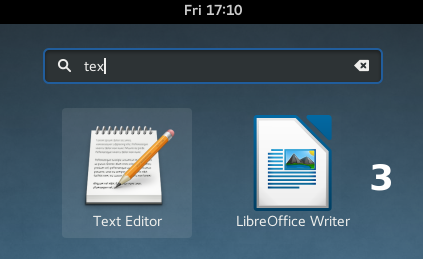
\includegraphics[width=0.72\textwidth]{img/search}
\captionbelow{Using the Search field} \label{fig:search}
\end{center}
\end{figure}

\item \emph{Virtual Workspaces} --- the vertical panel along the right side of the screen gives you an overview of your virtual workspaces. Virtual workspaces provide you with a convenient way to organize application windows rather than having all of them on a~single screen. In GNOME, you don't have a fixed number of workspaces available to you, but as many as you need. Whenever you drag an application window to an empty workspace, GNOME automatically adds a new empty one below it for you. It also automatically deletes surplus empty workspaces to make sure there is always exactly one without any windows in it.

You can use keybord shortcuts to move between virtual workspaces. Press $\keystroke{Ctrl}+\keystroke{Alt}+\keystroke{arrow $\uparrow$}$ to switch to the workspace directly above the current one, or $\keystroke{Ctrl}+\keystroke{Alt}+\keystroke{arrow $\downarrow$}$ to switch to the workspace directly below the one you are on.

\item The \emph{Preview of Open Windows} --- the middle part of the screen is used to give you an overview of all open windows. You can switch to a particular window by clicking on it with the left mouse button. If you prefer to use your keyboard, after entering the \emph{Activities Overview}, press \keystroke{arrow $\downarrow$} and then use arrow keys to navigate between the windows. Press \keystroke{Enter} to switch to the selected window.
\end{enumerate}

\section*{Adjusting System Settings}

To change system and user settings, open the \emph{All Settings} window either by selecting \emph{Settings} from the list of application launchers, or by typing \enquote{Settings} in the \emph{Search} field as described above.

\begin{figure}[tbp]
\begin{center}
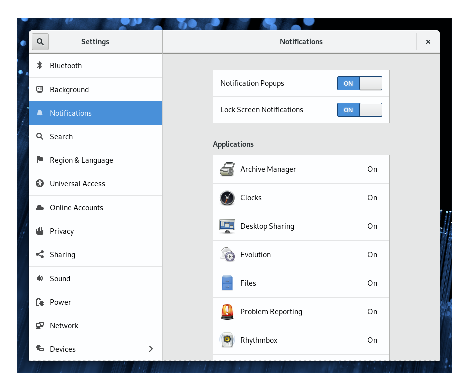
\includegraphics[width=0.72\textwidth]{img/settings}
\captionbelow{User and system settings} \label{fig:settings}
\end{center}
\end{figure}

Here you can configure anything from the desktop background and the system language to printers, network connections, and user accounts. You can also connect to different online accounts in cloud services such as Nextcloud, Google, and Facebook, and allow different desktop applications to access your data stored in those services. Do you use instant messaging and need to access your contacts? This way you will only need to log in to your cloud account once and all your contacts will be immediately accessible.

\section*{Installing Additional Software}

\emph{Fedora Workstation} includes a lot of commonly used applications in the default installation: \emph{Mozilla~Firefox} as the default web browser, \emph{LibreOffice} as the office suite, \emph{Videos} as a multimedia player, and many more. But what if you need something else?

Of course, not all software can be included in the default installation. Thousands of software packages are therefore readily available in so called \enquote{repositories} from which you can easily download them. Repositories are hosted on remote servers and their mirrors and provide packages of different applications and libraries. Have you heard of \emph{app stores} on mobile platforms? The basic principal is the same. If you want to download and install a program from the web, first check if it is not already available in the repositories. That's how you install most applications on Linux.


So how do you install additional software? Basically, you have two options:
\begin{enumerate}
\item Use the graphical application called \emph{Software} --- \emph{Software} offers exactly what you would expect from similar applications on mobile platforms: it is an elegant and easy to use gateway to repositories that allows you to search for applications and their add-ons, or browse applications from various categories. Each application has its own profile with a brief description, license, size information, and so on. And of course, all applications are open source and free to use.

In addition, \emph{Software} allows you to uninstall applications you no longer want on your system. You can also use it to update the system and installed packages.

\begin{figure}[htbp]
\begin{center}
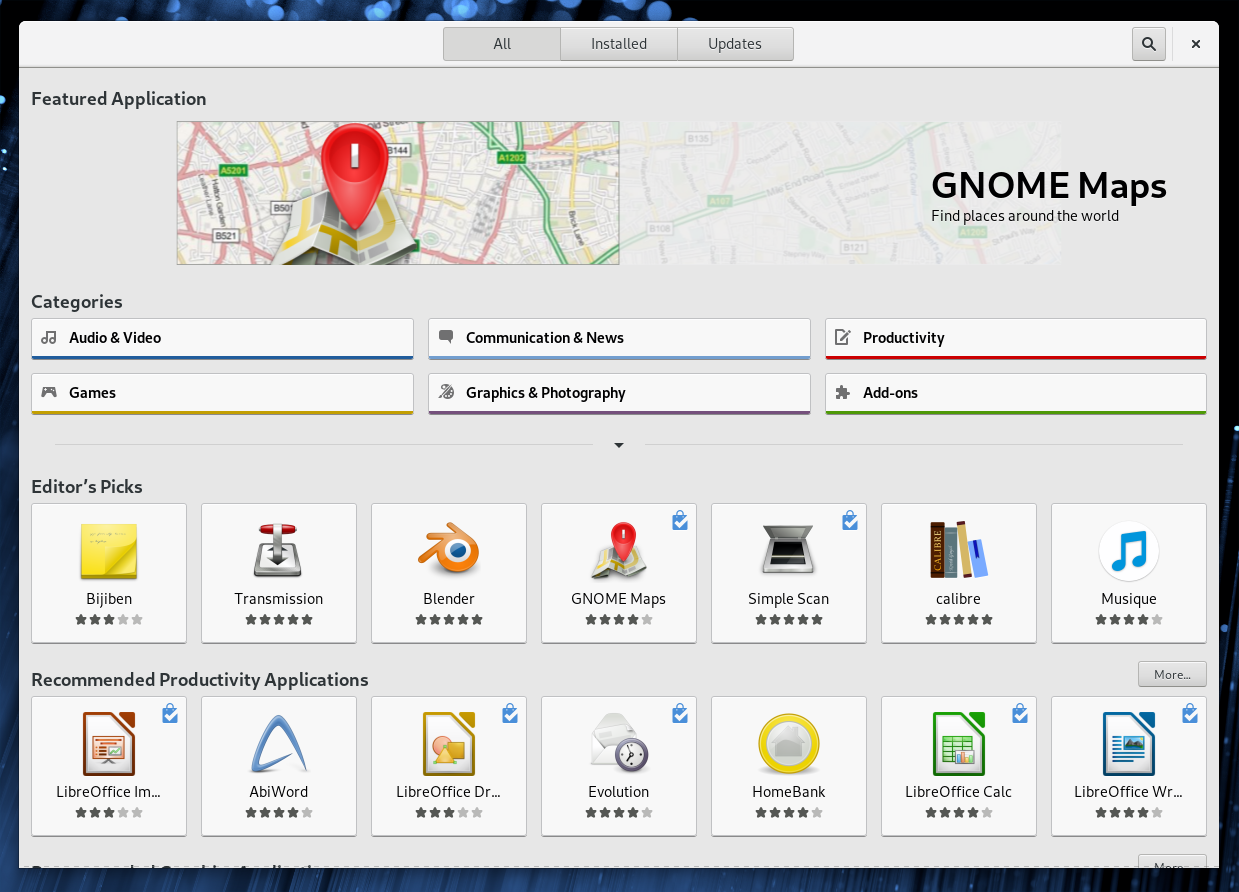
\includegraphics[width=0.72\textwidth]{img/software}
\captionbelow{Software management in Fedora} \label{fig:software}
\end{center}
\end{figure}

\item Use \emph{dnf} on the command line or its graphical interface  --- \emph{Software} allows you to search for and install desktop applications from the repositories, but will not offer you other types of packages, such as libraries, command-line tools, or documentation. Nevertheless, the Fedora repositories host almost 20,000 packages and most of them don't represent desktop applications. To find, install, uninstall, or update such packages, use the command-line tool called \emph{dnf} or its graphical interface called \emph{dnfdragora}, which will give you the comfort of desktop applications.
\end{enumerate}

\section*{Codecs and Other Software}

What if some software is not available in the Fedora repositories? This can happen, you may need a specific codec or a driver that can be distributed free of charge, but for various reasons (typically because of its license or patents) it can't be distributed by the \emph{Fedora Project}. That's where third-party repositories may come in handy.

Third-party repositories are not maintained by the \emph{Fedora Project} and are not associated with it in any way. It's important to note that the \emph{Fedora Project} is not liable for those software sources and cannot even guarantee that they will be in accordance with your local copyright and patent laws.

Typically, you will find four types of third-party repositories:
\begin{enumerate}
\item\emph{Vendor repositories} --- corporations such as Google or Adobe offer software sources that include their products, from development utilities to programs such as \emph{Google Chrome} and the \emph{Adobe Flash Player} plugin. A package installed from their website usually enables their repository in order to receive future updates. Once a repository is added to the software sources, you will be able to find the packages it provides by using already mentioned tools, \emph{Software} and \emph{dnf}. You can manage those packages like any other packages available from the official Fedora repositories.

\item\emph{Other repositories} --- there are several large third-party software sources with many packages that usually include software that is not open source or is patent-protected. For example, you may find multimedia codecs or specific drivers in repositories such as \emph{RPMFusion}. After you add the repositories, you install packages from them the same way you would install them from the official Fedora repositories.

\item\emph{Copr repositories} --- unlike in the previous cases, software in Copr repositories has always its license compatible with Fedora. Copr repositories are easy to add and are the biggest source of software for Fedora outside of the official repositories. They include the newest, often development versions of desktop environments, applications, and frameworks and you can find them at \url{copr.fedoraproject.org}.

\item\emph{Emerging universal app formats} --- recently, several formats, which are trying to unify application delivery across Linux distributions, have emerged. One of them is \emph{Flatpak} which is supported by default in \emph{Fedora Workstation}. Just like packaging systems \emph{Flatpak} allows multiple independent repositories, but most apps for \emph{Flatpak} reside at \url{flathub.org}.
\end{enumerate}

Before installing any packages from third party repositories, make sure that you understand what they change in your system. You should not blindly install software that is not officially shipped by the \emph{Fedora Project}, and you should always check if the source can be trusted and packages it provides won't do any harm to your system.
\endinput

\chapter*{How to Tweak Fedora Workstation?}
\section*{GNOME Shell Extensions}

\emph{GNOME Shell extensions} are an invaluable tool when it comes to customizing the system for your particular needs. There are hundreds of extensions that change individual elements of the user interface or add new ones. With these extensions, you can change the look and feel of various menus, icons, panels, indications, displays, window switching, and many other things.

You can explore them and install GNOME Shell extensions in \emph{Software} (under Addons/Shell Extensions), or directly in your web browser by visiting \url{extensions.gnome.org}.

Just keep in mind that the extensions can have an impact on the stability of your desktop. They're also third-party software the Fedora Project doesn't give any guarantees for. So be careful what extensions you enable, and if you experience any stability problems, disable them.

\section*{GNOME Tweaks}

Fedora also includes \emph{GNOME Tweaks}, a powerful utility that allows you to fine tune your desktop and change settings that are not available in the default configuration tool. With this utility, you can adjust the behavior of virtual workspaces, the behavior of the system during charging, application fonts, keyboard shortcuts, and much more. As a~matter of fact, you can even use GNOME Tweak Tool to manage the GNOME Shell extensions mentioned above.
\endinput

\chapter*{Where to Look for Further Information}

This handbook exists to help you get started with \emph{Fedora Workstation}. But, what can you do if you encounter a problem that you can't solve quickly? A good rule of thumb is to remember that any problem you're encountering has probably already been solved by somebody else before you. Here is where to look for solutions:
\begin{itemize}
\item\url{ask.fedoraproject.org} --- the official Q\&A forum with a large user base and a large archive of answered questions.

\item\url{fedoramagazine.org} --- articles from the Fedora world, including announcements and information about new applications.
\end{itemize}

\section*{What to Do If You Encounter a Bug}

It is possible that you will encounter a bug. What then? Fedora uses a bug tracker called Bugzilla that is provided by Red~Hat and you can find it online at \url{bugzilla.redhat.com}. Keep in mind that bugs must be reported in English.

Fedora also comes with a tool called \emph{ABRT} (Automatic Bug Reporting Tool). When a problem occurs, \emph{ABRT} detects it and allows you to report a bug by just agreeing to share the details with the \emph{Fedora Project}.

Reporting bugs is a great way to contribute to Fedora and help us make it better.

\section*{Fedora Editions}

Unlike many other Linux operating systems, Fedora consists of three main editions. In addition to the \emph{Workstation} edition, which is described in this guide, there are also \emph{Server} and \emph{Atomic} editions:
\begin{itemize}
\item The \emph{Server} edition is designed for server uses, and features applications like \emph{Cockpit} which allows for easy remote management of servers through a web browser.

\item The \emph{Atomic} edition is a minimal version of Fedora optimized for deploying containers. It uses \emph{OStree} to provide atomic updates.
\end{itemize}

\section*{Fedora Spins}

Everything in this guide is about the default \emph{Fedora Workstation} edition, which uses \emph{GNOME~3} and \emph{GNOME Shell}. Because there are many other popular desktop environments, so called spins offer alternative software builds of Fedora with these environments. Do you prefer the \emph{KDE Plasma Desktop}? You'll find an installation image with it. \emph{Xfce}? \emph{LXDE}? We have prepared installation images for everything. You don't have to reinstall your whole system from a spin image if you want to try a different environment, but spin images come with everything preconfigured by default.

But we don't have to stop with Fedora spins. The ARM architecture is currently the most used mobile platform and is the platform of choice for development boards like Banana Pi, BeagleBone, or the Raspberry Pi. There are images built to run on these kinds of systems too in the form of server versions or minimal installation images.
\endinput


\backmatter
\renewcommand*{\chapterpagestyle}{empty}

\newpage\null\thispagestyle{empty}\newpage

\newpage\null\thispagestyle{empty}\newpage

%\cleardoubleplainpage
\pagenumbering{gobble}
\newpage\mbox{}\newpage
\begin{center}

{\it\large Fedora Workstation -- A Beginners Guide}

\bigskip

{\it Project Lead:}

Jiří Eischmann

{\it Czech Language Authors:}

Lukáš Kotek, et. al.

{\it Czech Language Proofreading:}

Květa Mrštíková and Jiří Kroupa

{\it English Language Proofreading and Authors:}

Brian Exelbierd and Jaromír Hradílek

{\it Typography and Layout:}

Petr Čech

{\it Cover Design::}

Maria Leonova

{\it First Edition Released in September 2015.

Released under CC BY-SA 3.0}
\end{center}



\end{document}
\endinput
